\section{Lateral Control}
\label{lateral_control}

Chapter \ref{longitudinal_control} discussed  some basic longitudinal control techniques used in autonous vehicles
In this chapter, we will go through the lateral control. Concretely, in this chapter we will discuss the following

\begin{itemize}
\item Geometric path following
\item Model predictive control or MPC
\end{itemize}

On the one hand, the control strategies based geometry are built on the no-slip assumption introduced when we were discussing kinematic modeling namely in chapter \ref{vehicle_kinematics_and_dynamics}.
On the other hand, MPC is an example of an advanced control strategy regularly used in autonomous vehicles.

However, we will begin with some core concepts needed to perform lateral control and define different types of
reference path and how to compute heading and crosstrack errors relative to those reference paths.  

\subsection{The reference path}

One of the main concerns in autonomous vehicles is ensuring the vehicle can precisely
follow a predefined path, executing the motion plan devised in the higher level
planning module. This is the main goal of lateral control which must select
the steering angle required to correct any errors that accumulate and track changes in the path
direction as they appear. In order to be able to design the lateral controller, we need to define the error between the vehicle position and the
appropriate desired path coordinates, select a control design strategy that drives errors to zero while still satisfying
steering angle limits, and consider the dynamic limitations of vehicle and desired ride characteristics such as maximum lateral acceleration and minimum jerk. 
Control command must be cognizant of the available tire forces and not exceed the capabilities of the vehicle when correcting
for tracking errors. The reference path is a fundamental interface between the planning system in the lateral controller, and can be defined in multiple ways, see Figure \ref{reference_path_1}. 


\begin{figure}[!htb]
\begin{center}
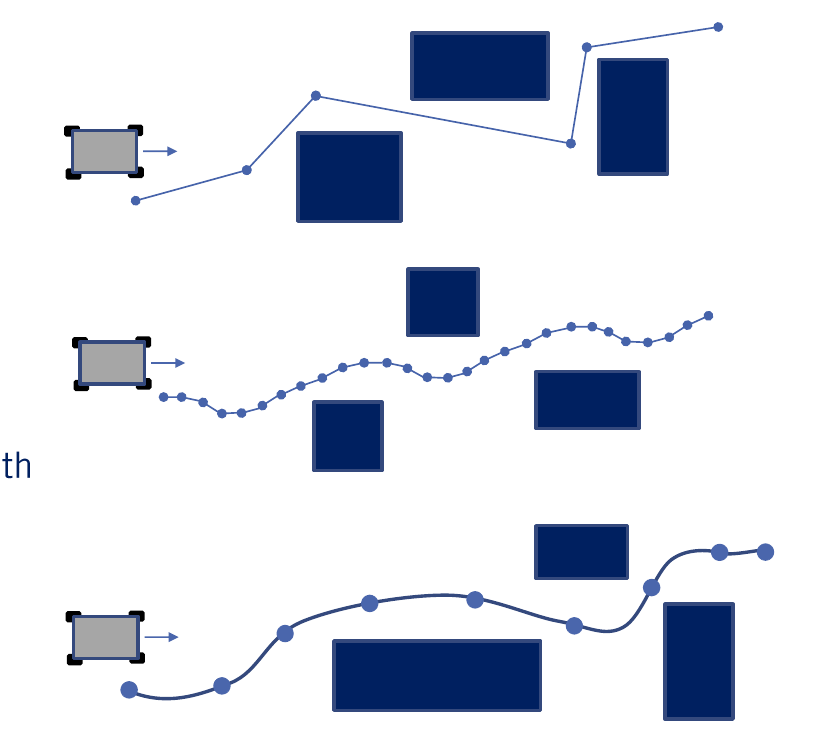
\includegraphics[scale=0.380]{img/lateral_control/reference_path_1.jpeg}
\end{center}
\caption{Reference path definitions.}
\label{reference_path_1}
\end{figure}

\textbf{Sequence of straight line segments}

The easiest approach is to define a sequence of straight line segments by requiring a sequence of end point vertices
that are connected linearly. This path definition can be very compact and easy to construct, assuming points are well spaced and the environment allows for
mostly straight line motion, as in a Manhattan grid of roadways. However, the path includes heading discontinuities, which make precise tracking
a challenge with a steered vehicle. 

\textbf{Series of tightly spaced waypoints}

A refinement of the line segment approach is to provide a series of tightly spaced waypoints. This spacing is usually fixed in
terms of distance or travel time. The relative position of the waypoints can be restricted to satisfy
an approximate curvature constraint. Waypoint paths are very common, as they are easy to work with and
can be directly constructed from state estimates or GPS waypoints collected in earlier runs
of a particular route. 

\textbf{Continuous parametrized curves}

It is also possible to define a path using a sequence of continuous
parameterized curves, which can be either drawn
from a fixed set of motion primitives or can be identified through
optimization during planning. These curves provide the benefit
of continuously varying motion, and can be constructed to have
smooth derivatives to aid in the consistency of error and
error rate calculations. 



In all cases of path following, the controller tries to eliminate
the offset of the vehicle to the desired path and to align the vehicle heading
with the path heading. For each of these paths definitions, the direction of travel along
the path is also provided, which can be encoded with the
point ordering or curve ordering. We will define
these two terms shortly, as they both play a critical role in the design of lateral controllers. Let's now introduced
the two main categories of lateral control design, which are widely used
in autonomous vehicles. 

The first category of controllers
are geometric controllers, which rely on the geometry
and coordinates of the desired path and the kinematic models of the vehicle. We'll consider two types
of controllers that are geometric controllers:

\begin{itemize}
\item The pure pursuit controller 
\item The Stanley controller
\end{itemize}

We'll look at these in detail in
the next lessons in this module. The other category of controllers
is called dynamic controllers. The most popular
advanced controller in this category is the model
predictive controller or MPC, which performs a finite
horizon optimization to identify the control
command to apply. MPC is commonly used because of its ability to handle
a wide variety of constraints and to identify optimized solutions that consider more than just the current errors. 


\subsubsection{Errors in path tracking}
\label{error_path_tracking}

 Let's now investigate the definitions of errors in path tracking control. We'll use the kinematic bicycle model as our basis for this discussion. So, let's quickly review the important parameters
of the bicycle model. The bicycle model is a suitable control oriented model of a four-wheel vehicle, where the front left
and right wheels are combined into a single steerable wheel, and the rear left and right wheels are combined together in
a single drive wheel. For this discussion, we'll use a line segment as our reference path, shown as a solid black line
in Figure \ref{reference_path_2}. 

\begin{figure}[!htb]
\begin{center}
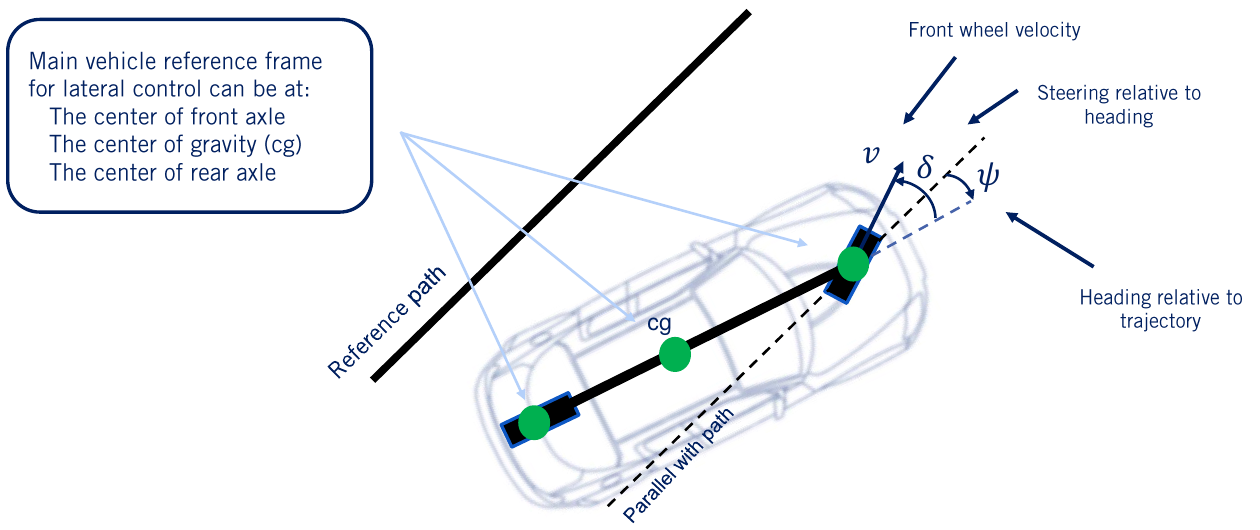
\includegraphics[scale=0.280]{img/lateral_control/reference_path_2.jpeg}
\end{center}
\caption{Reference path definitions.}
\label{reference_path_2}
\end{figure}

A dashed black line that is parallel to the path but runs through the center of the front axle is also visible. 
For the purposes of lateral control, we redefine our heading relative to the current path line segment. The variable side will
be reused to represent the relative heading angle of the vehicle with respect
to the path line. The front wheel velocity $V$ and the steering angle $\delta$ relative to the heading direction 
do not change, and are also shown in the Figure. 


\begin{framed}
\theoremstyle{remark}
\begin{remark}{}

Note that we can place
a reference frame for the vehicle at the center
of the rear axle, at the center of the front axle, or at the center of gravity
depending on our controller design.
\end{remark}
\end{framed}

As mentioned in the previous section, we'll introduce two types of error:

\begin{itemize}
\item Heading error 
\item Crosstrack error
\end{itemize}

\textbf{Heading error}

The heading error is equal to the difference between path heading and vehicle heading at
the reference point along the path. It is a principal measure of how well the vehicle is aligned with and moving in
the direction of the desired path. The rate of heading error $\dot{\psi}$ helps us understand how the heading
error evolves over time, and can be computed from the kinematic bicycle model equations. The rate of heading error
can be expressed in terms of any of the three vehicle reference points as well. Figure \ref{heading_error_def} summarizes this.

\begin{figure}[!htb]
\begin{center}
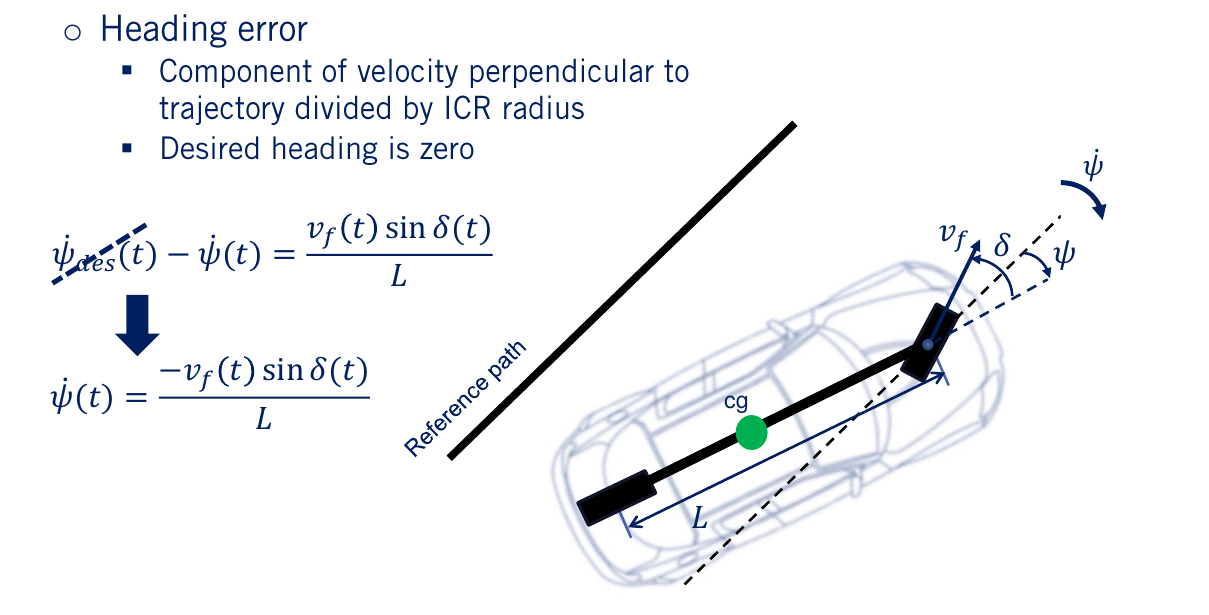
\includegraphics[scale=0.280]{img/lateral_control/heading_error_def.jpeg}
\end{center}
\caption{Definition of heading error.}
\label{heading_error_def}
\end{figure}

Here we present the rate of heading error relative to the front axle, as will be used in the Stanley controller discussed later. For straight line segments, the desired heading rate
of change is zero, and it can be removed. This is because the reference heading is not time-varying for a straight line, and is in fact equal to zero, 
as we have redefined our heading relative to the current path direction. 

\textbf{Crosstrack error}

The other type of error is an offset error called
the crosstrack error. The crosstrack error is the distance between
the reference point on the vehicle and the closest point
on the desired path, see Figure \ref{crosstrack_error_def}. 

\begin{figure}[!htb]
\begin{center}
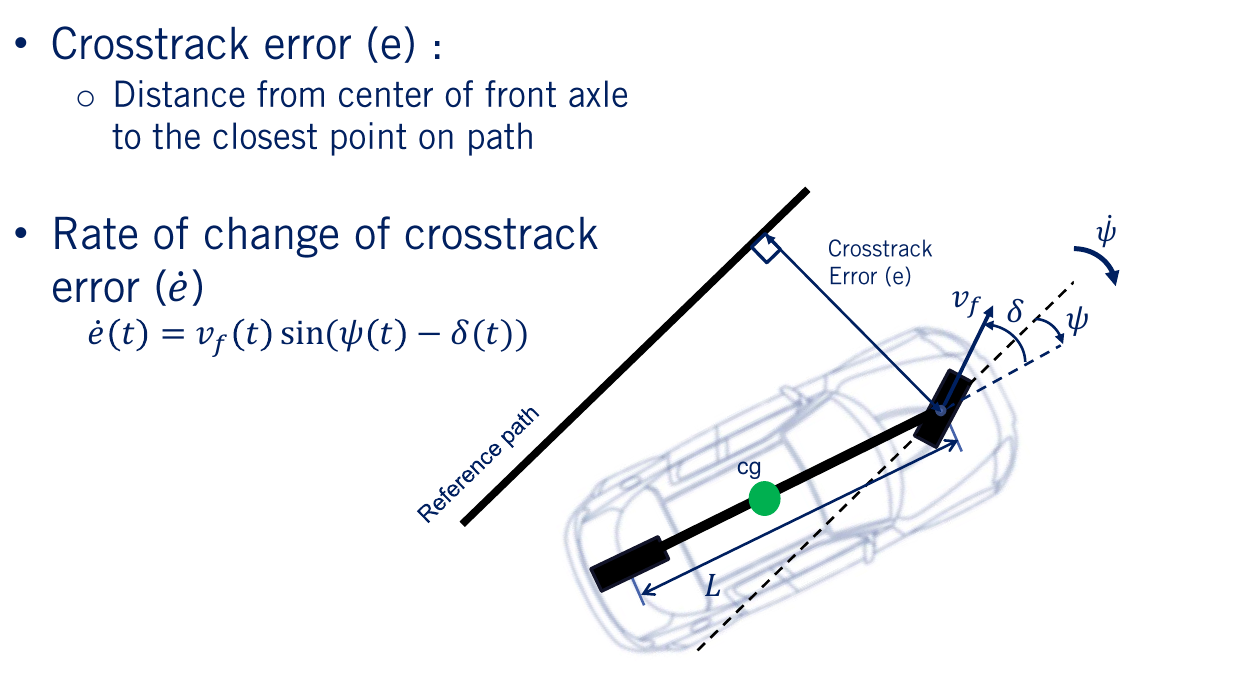
\includegraphics[scale=0.280]{img/lateral_control/crosstrack_error_def.jpeg}
\end{center}
\caption{Definition of crosstrack error.}
\label{crosstrack_error_def}
\end{figure}

It is the principal
measure of how close the vehicle's position is to
the desired position along the path. Both heading error and crosstrack
error must converge to zero for the vehicle to be properly
tracking the desired path. The line from the vehicle
reference point to the path reference point is
perpendicular to the path. The rate of change of the
crosstrack error can be calculated by extracting the lateral component
of the forward velocity. From this equation, we can see
that as the velocity increases, the crosstrack error
changes more quickly, meaning that smaller steering
angles are needed to correct for the same size
crosstrack errors. 

\subsection{Heading and crosstrack errors for curved paths}
TO BE FILLED see \cite{WangH2002}


Extending this discussion
of the heading and crosstrack errors to the curved paths adds some additional complexity, as it is not immediately clear where the reference point on
the curved path should lie. The geometric relations required fall outside the scope of this video. We've nonetheless provided links
in the supplemental materials for those interested in error calculations relative to curved paths. 

\subsection{Geometric steering control: Pure pursuit}
\label{geometric_steering_control_pure_pursuit}

We'll first introduce the concept of a geometric path tracking controller which relies on our kinematic vehicle model for selecting steering commands and then we'll design a pure pursuit controller for our self-driving cars to track a reference path through the environment. Let's get started. 

\begin{framed}
\theoremstyle{remark}
\begin{remark}{\textbf{What is a geometric path tracking controller?}}

Generically, it is any controller that tracks a reference path using only the geometry of the vehicle kinematics and the reference path
\end{remark}
\end{framed}

In the case of self-driving cars, a geometric path tracking controller is a type of lateral controller that ignores 
dynamic forces on the vehicles and assumes the no-slip condition holds at the wheels. 
It relies on a kinematic bicycle model and the error measures defined in the previous section to construct a steering command rule that achieves path tracking. 
Because of its simple nature, it is very popular and useful in robotics and autonomous driving. 

However, this simple approach has a downside in that its performance suffers when the vehicle motion does not match 
the no-slip assumption, as is the case in aggressive vehicle maneuvers with high lateral acceleration. 
In these cases, a deeper understanding of the limits of the available tire forces is needed, as are 
more involved control strategies. 

When the vehicle is operating in the linear tire region and a tire is not saturated, however, 
geometric path tracking controllers can work very well. 

Geometric path tracking controllers rely on a reference point along the desired path, which can be the same reference 
point used to compute heading and cross track errors, or it can be a look-ahead point some distance in front of the vehicle along the path, 
an example of which is shown in red in Figure \ref{look_ahead}. 

\begin{figure}[!htb]
\begin{center}
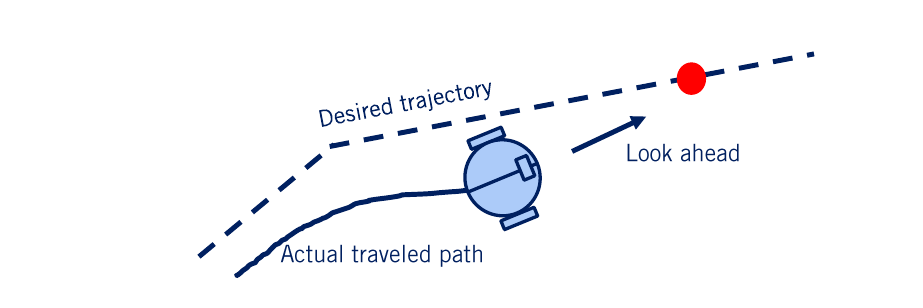
\includegraphics[scale=0.280]{img/lateral_control/look_ahead.jpeg}
\end{center}
\caption{Look-ahead point illustration.}
\label{look_ahead}
\end{figure}

In fact, the pure pursuit controller we're about to derive uses a look-ahead point on the reference path, 
while the Stanley controller uses the same reference point as is needed for error calculations. 
Let's now take a closer look at the pure pursuit controller. 

In the pure pursuit method, the core idea is that a reference point can be placed on the path a fixed distance ahead of the vehicle, 
and the steering commands needed to intersect with this point using a constant steering angle can be computed. 
As the vehicle turns towards the path to follow this curve, the point continues to move forward, 
reducing the steering angle and gently bringing the vehicle towards the path. 
In this method, the center of the rear axle is used as the reference point on the vehicle, and we define the line that connects 
the center of the rear axle to the target reference point as a line of fixed distance $l_d$, known as the look-ahead distance, which is the red dashed line in  Figure \ref{pure_pursuit}. 

\begin{figure}[!htb]
\begin{center}
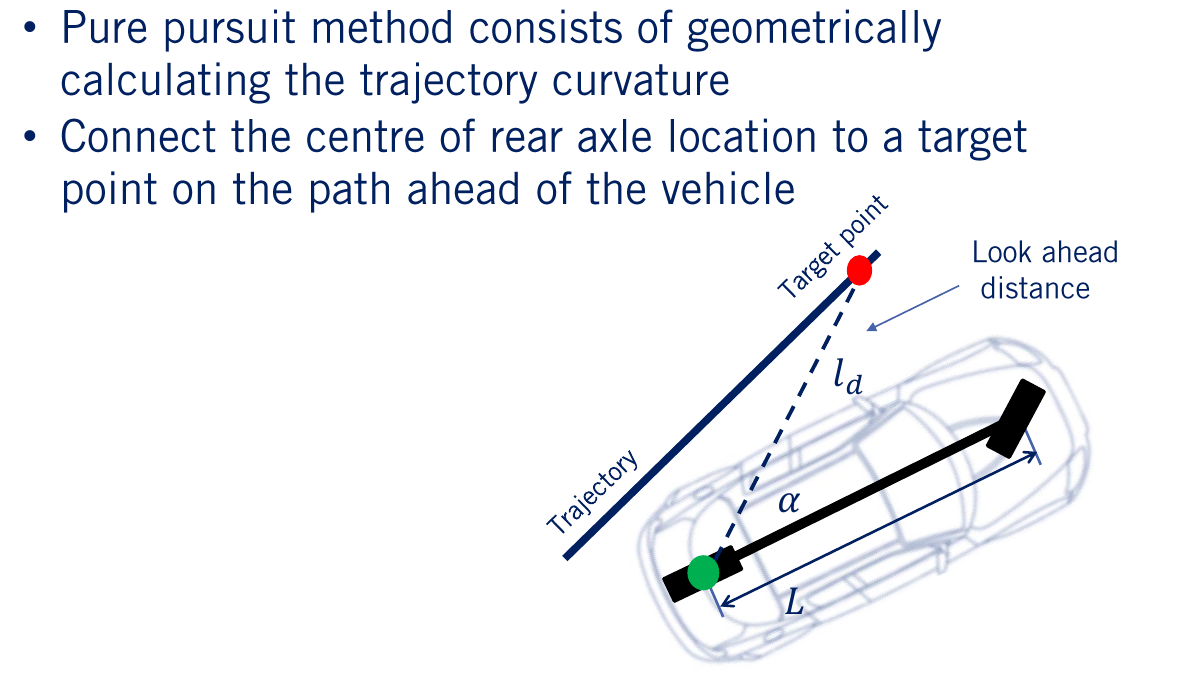
\includegraphics[scale=0.280]{img/lateral_control/pure_pursuit.jpeg}
\end{center}
\caption{Pure pursuit.}
\label{pure_pursuit}
\end{figure}

The angle between the vehicle's body heading and the look-ahead line is referred to as $\alpha$. In order to construct the pure pursuit controller, 
we once again turn to the concept of the instantaneous center of rotation ICR. 
The target point on the trajectory, the center of the rear axle, and the instantaneous center of rotation form a triangle with two sides of length $R$ and one of length $l_d$. 

\begin{figure}[!htb]
\begin{center}
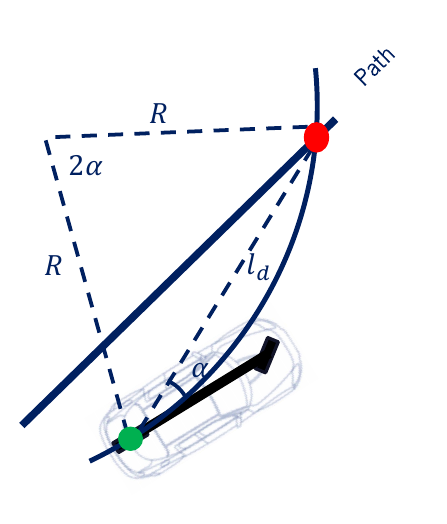
\includegraphics[scale=0.280]{img/lateral_control/pure_pursuit_form_1.jpeg}
\end{center}
\caption{Pure pursuit formulation.}
\label{pure_pursuit_form_1}
\end{figure}

We'd like to define the arc that takes the vehicle reference point to the target point on the path. 
This arc is the part of the ICR circle that covers the angle of $2\alpha$. The angle $2\alpha$ can be derived using standard trigonometric identities. 
Based on the law of sines, we can write the following equation: 

\begin{equation}
\frac{l_d}{\sin(2\alpha)} = \frac{R}{\sin(\frac{\pi}{2} - \alpha)} 
\end{equation}

Then using some more trigonometric identities, we can simplify the equations as follows, 

\begin{equation}
\frac{l_d}{2\sin(\alpha)\cos(\alpha)} = \frac{R}{\cos(\alpha)} 
\end{equation}

which leads to the compact expression 

\begin{equation}
\frac{l_d}{\sin(\alpha)} = 2R 
\end{equation}

Finally, the curvature $\kappa$, which is the inverse of the arc radius $R$, is equal to:

\begin{equation}
\kappa = \frac{1}{R} = \frac{2\sin(\alpha)}{l_d}
\label{curvature_eq_1}
\end{equation}

Now, let's take a look at the bicycle model to calculate the steering angle $\delta$ needed to track this arc. 
Recall that the steering angle defines the arc radius and yields the relation

\begin{equation}
\tan(\delta) = \frac{L}{R}
\end{equation}

Combining this expression with the expression for $R$ derived earlier, we can now express the steering angle needed to follow the arc in terms of easily computed values. 
The steering angle $\delta$ is set to 

\begin{equation}
\delta = \arctan(\frac{2L\sin(\alpha)}{l_d}
\end{equation}

This is an easily implemented controller for steering, but how well will it perform? To understand this, we need to dig into how the error values evolve in closed loop. 
For the pure pursuit controller, we can define the cross track error as the distance between the heading vector and the target point. 
Once again, we'll use $e$ to denote the cross track error, see Figure \ref{pure_pursuit_form_2}. 

\begin{figure}[!htb]
\begin{center}
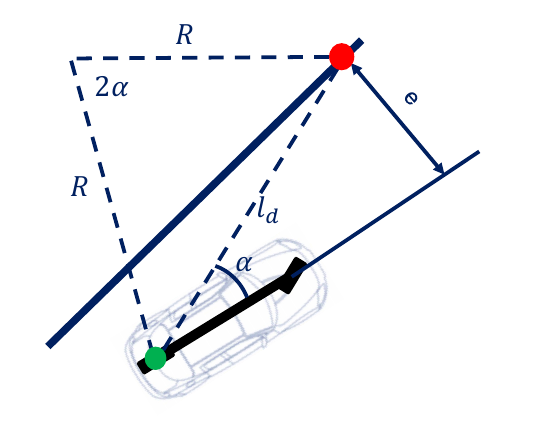
\includegraphics[scale=0.280]{img/lateral_control/pure_pursuit_form_2.jpeg}
\end{center}
\caption{Crosstrack error.}
\label{pure_pursuit_form_2}
\end{figure}

We now arrive at the expression

\begin{equation}
\sin(\alpha) = \frac{e}{l_d}
\end{equation}

Combining this with the expression for curvature, i.e. equation \ref{curvature_eq_1}, shows us that the curvature of the path created by the pure pursuit controller is proportional to the cross track error at the look-ahead reference point.

\begin{equation}
\kappa = \frac{e}{l_{d}^2}
\label{curvature_eq_2}
\end{equation}

As the error increases, so does the curvature, bringing the vehicle back to the path more aggressively. This equation demonstrates that the pure pursuit controller works in a manner similar to proportional control to correct cross track error using path curvature as the output of the controller. The proportional gain depends on 

\begin{equation}
\frac{2}{l_{d}^2}
\end{equation}

So as the look-ahead distance increases, the proportional gain decreases in a nonlinear manner. It's important to note that the pure pursuit controller with a fixed value of $l_d$ leads to a curvature controller that does not take into account the vehicle speed. This means that the selected steering angle would be the same regardless of whether the vehicle is going 10 kilometers per hour or 100 kilometers per hour, leading to very different lateral acceleration's. A controller tuned for high-speed would be far too sluggish at low speed, and one tuned for low speed would be dangerously aggressive at high speeds. To overcome this limitation, we add one more modification to our pure pursuit controller. We can vary the look-ahead distance $l_d$ based on the speed of the vehicle. We define the look-ahead distance to increase proportional to the vehicle forward speed. The addition to the controller takes the form

\begin{equation}
l_d = K_{dd}v_f
\end{equation}

where $v_f$ is the forward velocity. Substituting this adjustment into the steering angle command equation, we arrive at the complete pure pursuit controller. 
The controller selects the steering angle that will form an arc to the look-ahead reference point, and adjusts this look-ahead point to be further away the faster the vehicle is traveling. 

\begin{equation}
\delta = \arctan(\frac{2L\sin(\alpha)}{K_{dd}v_f}
\end{equation}

This design results in steering commands and turn rates that are achievable given available tire forces, although it must be tuned to do so. You now are ready to start building geometric lateral controllers for self-driving cars. 

In this section, we defined the class of geometric path tracking controllers and derived the pure proceed controller.
In the next section, we'll explore the second geometric path tracking controller, the Stanley controller. 

\subsection{Geometric steering control: Stanley controller}
\label{geometric_steering_control_stanley_controller}

In section \ref{geometric_steering_control_pure_pursuit}, we derived the pure pursuit controller, a geometric path tracking controller 
that defined steering input based on a look ahead reference point. In this section, we will cover a second geometric path tracking controller, the Stanley controller. 
This controller was used by the Stanford racing team to win the second Darpa Grand Challenge event. 
Specifically in this section, we will derive the Stanley geometric controller, analyze the evolution of its steering commands 
for small and large errors, and evaluate the control performance in the form of convergence to the desired path 
from arbitrary starting conditions. 

\subsubsection{The Stanley controller}

The Stanley controller is a geometric path tracking controller which is simple but useful for autonomous robotics and autonomous cars. 
The method was originally developed by Gabe Hoffman at Stanford University as 
his contribution to the winning teams entry, and is named after the vehicle Stanley. 

The main concept that went into the creation of the Stanley controller was that a change in the reference position could lead to different, 
possibly more desirable properties of the control. Dr. Hoffman was seeking a control law with global convergence to the path and predictable 
decay of the errors that would be independent of vehicle speed. So, Dr. Hoffman switched the vehicle reference point used for the controller 
to the center of the front axle instead of either the CG or the rear axle to see how this new controller might behave. 
The next modifications he added were to consider both heading alignment and cross track error without a look-ahead distance, 
but directly at the reference point. Finally, the Stanley controller caps its outputs to fall within the limits of the maximum steering angle. 
In all these three considerations formed the basis for the resulting control law. 

Let's define each of the terms of the Stanley controller. In Figure \ref{stanley_control}, you can see the slight modifications to the relevant terms based on the Stanley assumptions. 

\begin{figure}[!htb]
\begin{center}
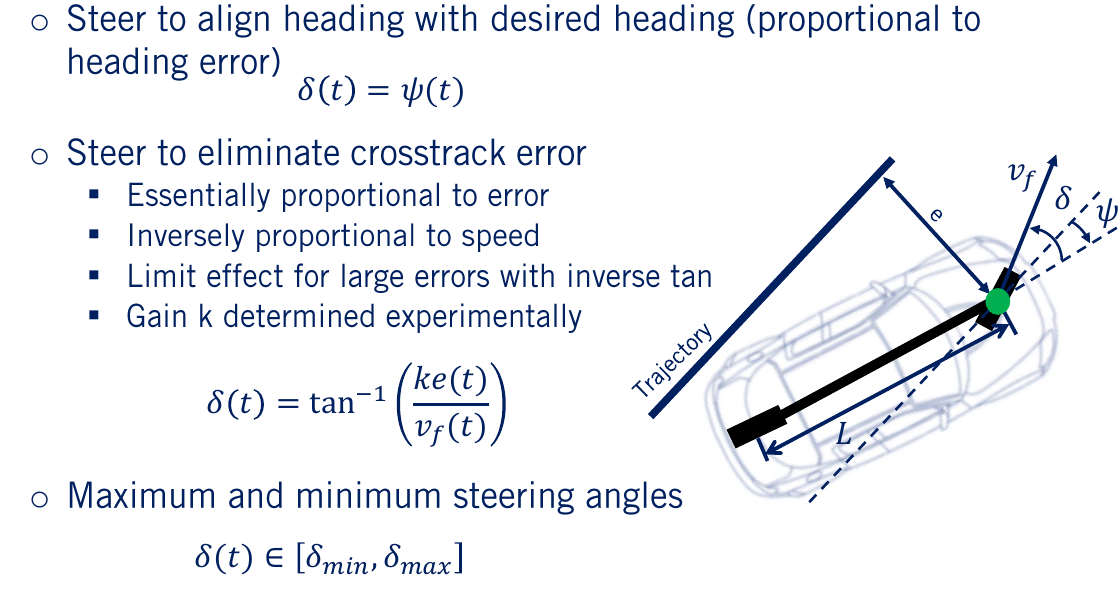
\includegraphics[scale=0.280]{img/lateral_control/stanley_control.jpeg}
\end{center}
\caption{Stanley control.}
\label{stanley_control}
\end{figure}

The cross track error is measured relative to the front axle, and the reference point on the path has no look ahead distance associated with it. 
Let's make each of the three components of the Stanley controller more concrete. 
First, to eliminate heading error relative to the path, the steering angle is set equal to the heading directly. 
\begin{equation}
\delta(t) = \psi(t)
\end{equation}
Then to eliminate cross track error, a proportional control is added, whose gain is scaled by the inverse of the forward velocity. 
The control is then passed through an inverse tangent function 

\begin{equation}
\delta(t) = \arctan(\frac{ke(t)}{v_f(t)}
\end{equation}

which maps the proportional control signal to the angular range of

\begin{equation}
 [-\pi, \pi] 
\end{equation}

Finally, the steering angle command is kept to fall within the minimum and maximum steering angles, 

\begin{equation}
\delta(t) \in [\delta_{min}, \delta_{max}] 
\end{equation}
which are usually symmetric about 0. 

The similarities with the pure pursuit controller are not surprising, as both are seeking to perform the same task with the same kinematic model. 
The Stanley controller scales its gains by the forward speed in the same way as pure pursuit control, and also has the same inverse tangent of the proportional control signal. 
However, the independent penalization of heading and cross track errors and the elimination of the look-ahead distance make this a different approach from pure pursuit. 
The final control law simply combines these three elements to set the steering angle of the car as follows. 

\begin{equation}
\delta(t) = \psi(t) + \arctan(\frac{ke(t)}{v_f(t)}, ~~\delta(t) \in [\delta_{min}, \delta_{max}]
\end{equation}

Let's now take a look at what's steering angle is requested for different error signals. For heading error, the steering command points in the opposite direction to the heading error, causing the vehicle to turn to correct the misalignment with the path. 

\begin{figure}[!htb]
\begin{center}
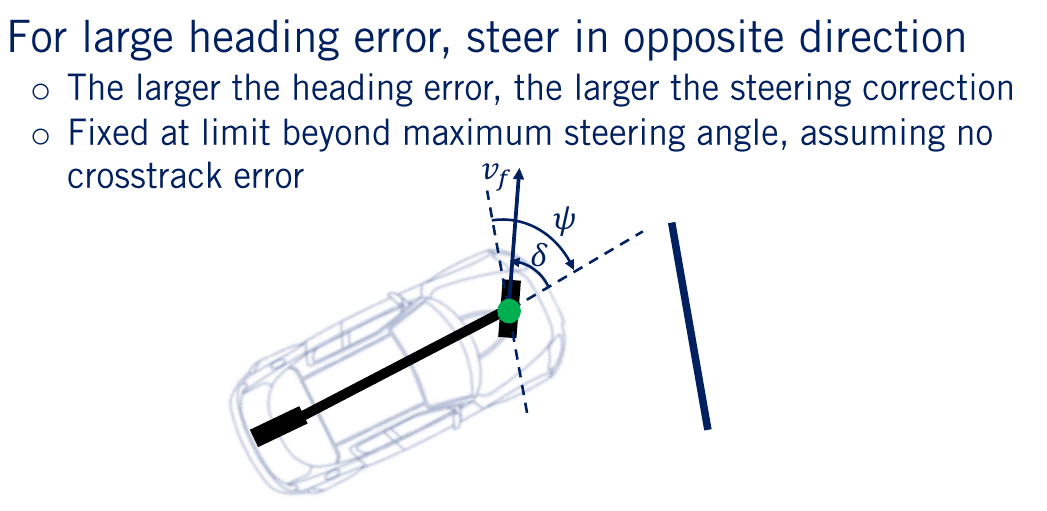
\includegraphics[scale=0.280]{img/lateral_control/stanley_control_2.jpeg}
\end{center}
\caption{Stanley control.}
\label{stanley_control_2}
\end{figure}

For large heading errors, for example, if the heading error exceeds the maximum steering angle, this part of the controller requests the maximum steering command until alignment falls back within the available balance. For large positive cross track error, $ke(t)/v_f$ becomes large and the inverse tangent approaches $\pi/2$. So we can approximate the Stanley control law as the heading error plus $\pi/2$. This large value clamps the steering command to the maximum and the vehicle turns towards the path. The effect of this term is to increase the heading error in the opposite direction, and so the steering command will drop to 0 once the heading error reaches $-\pi/2$. 
The vehicle then proceeds straight to the path until the cross track error decreases. At this point, the heading term starts correcting the alignment with the path again and ultimately, the vehicle starts to track the path more closely. 

\begin{figure}[!htb]
\begin{center}
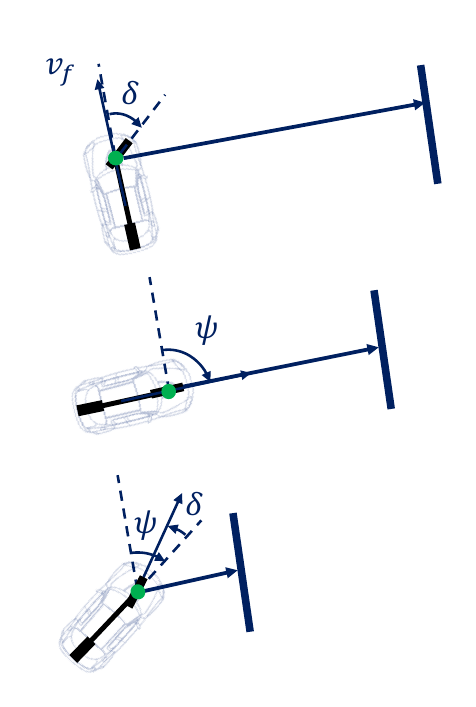
\includegraphics[scale=0.280]{img/lateral_control/stanley_control_3.jpeg}
\end{center}
\caption{Stanley control.}
\label{stanley_control_3}
\end{figure}

But how does this control actually converge to the path? 

As it turns out, it's possible to use our expression for the cross track aerodynamics defined in section [REF SECTION] of this module to get a sense for the convergence characteristics of the Stanley controller. Recall that the rate of change of the cross track error for a front axle reference point is equal to:

\begin{equation}
\dot{e}(t) = -v_f(t)\sin(\psi(t)-\delta(t)) = -v_f(t)\sin(\arctan(\frac{ke(t)}{v_f(t)}))
\end{equation}
which can be simplified to

\begin{equation}
\dot{e}(t) = \frac{-ke(t)}{\sqrt{1 + (\frac{ke(t)}{v_f})^2}}
\end{equation}

For small cross track errors we can further simplify to

\begin{equation}
\dot{e}(t) \approx -ke(t)
\end{equation}

This leads to the realization that the cross track error evolution follows a first-order differential equation, and the solution for this ODE is an exponential. Since $k$ is positive, we see that the error decays exponentially to 0. The most interesting aspect of this investigation is that the decay rate is completely independent of the speed. So faster vehicles will travel farther while converging to the path, but will converge to the path at the same time as slower moving vehicles. 

Let's now dive into a simulation example of the error dynamics for the Stanley controller to observe its convergence characteristics. In this example, let's take a look at two extreme scenarios, large initial cross track error and large initial heading error. In the first case, for large initial cross track error, let's assume the initial cross track error, $e(t)$ is $5m$, and that the maximum allowable steering angle $\delta_{max}$, is 25 degrees and the forward velocity, $v_f$, is $5m/sec$. We'll set the vehicle wheel base length $L$ to $1m$ for simplicity and the gain $k$ will be set to a value of 2.5. This was selected based on chosen parameters for the simulation and some trial and error testing. 

Figures \ref{stanley_control_4} and \ref{stanley_control_5} shows the results of the simulation

\begin{figure}[!htb]
\begin{center}
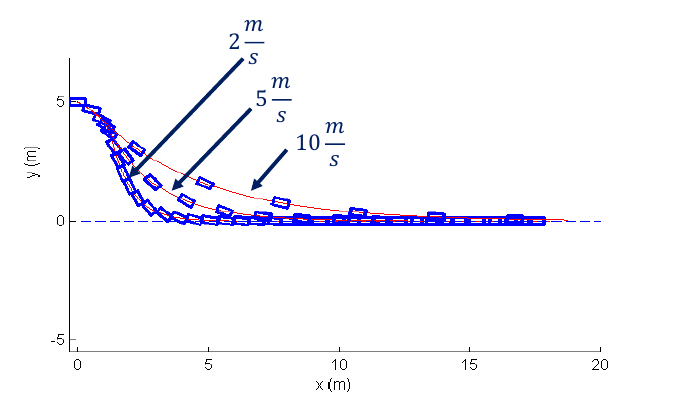
\includegraphics[scale=0.280]{img/lateral_control/stanley_control_4.jpeg}
\end{center}
\caption{Stanley simulation example.}
\label{stanley_control_4}
\end{figure}
\begin{figure}[!htb]
\begin{center}
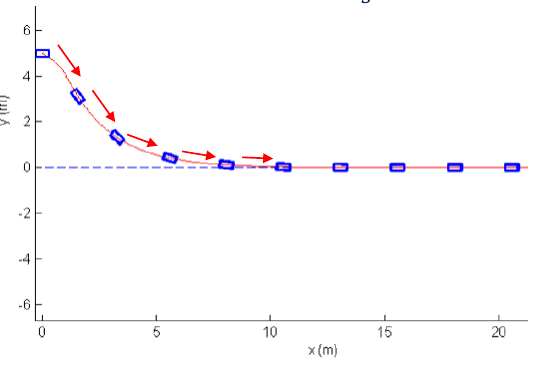
\includegraphics[scale=0.280]{img/lateral_control/stanley_control_5.jpeg}
\end{center}
\caption{Stanley simulation example.}
\label{stanley_control_5}
\end{figure}

The simulation shows how the Stanley controller corrects for a large cross track error and converges to the desired path. 
The large initial error leads to a large steering command that quickly turns the vehicle towards the path. 
The heading error and cross track error terms then reach an equilibrium, and the vehicle continues in a straight line towards the path. 
As the cross track error decreases, the exponential decay to the path becomes visible. Finally, the vehicle safely tracks the path in the final stages of the simulation. 
We can also run the same simulation at different forward velocities. So, let's try speeds of 2, 5 and 10 meters per second. The results show the main characteristics of the Stanley controller. In all cases, the turn towards the path, straight line progress and then exponential decay to the path are visible. 
The higher the speed, the further the car travels before reaching the path. 
However, the final convergence for small cross track errors takes the same amount of time in each case. 

In the second case, the simulation can be regenerated for the scenario at a large initial heading error. The parameters are the same as the previous case but the vehicle starts out on the path pointing very much in the wrong direction. Figure \ref{stanley_control_6} shows the simulation results. 

\begin{figure}[!htb]
\begin{center}
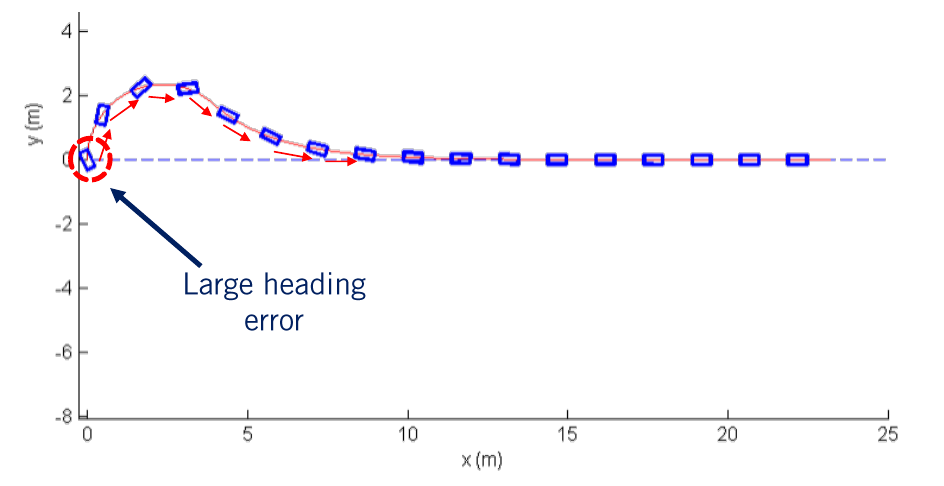
\includegraphics[scale=0.280]{img/lateral_control/stanley_control_6.jpeg}
\end{center}
\caption{Stanley simulation example.}
\label{stanley_control_6}
\end{figure}

The simulation results show the heading error is corrected by the Stanley control law. First, the steering command is up against its limit as the heading error is corrected. 
Then as the cross track error starts to grow, the steering commands continue to correct the heading of the car beyond the alignment with the path. Finally, the car enters the exponential convergence segment as before. These simulation results give us a good idea of the ability of the Stanley controller to correct arbitrarily large errors. 
In fact, it comes with a global stability proof, meaning that no matter what the initial conditions, the controller will guide the car back to its path. 
In practice however, the Stanley controller is still a geometric path tracking controller, and as such does not consider many different aspects of real self-driving car. 
For example, it does not consider noisy measurements, actuator dynamics or tire force effects, all of which can cause undesirable ride characteristics during maneuvers. 
It is possible, however, to make a few adjustments to the geometric path tracking controllers that help mitigate some of these most undesirable effects. During low-speed operation, the pure pursuit and Stanley controllers can behave quite aggressively when confronted with noisy velocity estimates. Since the velocity term is in the denominator of the fraction inside the inverse tangent, errors in low speed estimates tend to get amplified in the steering command. This leads to wild swings in the steering wheel, which is not desirable for rider comfort. So to get rid of this issue and to increase the stability of our solution at low speeds, we add a positive softening constant that ensures the denominator always has a minimum value. This softening constant can be tuned in the field. At higher speeds, we have the issue that steering commands need to vary slowly to ensure lateral forces are not excessive. Even with this scaling on speeds, Stanley's response was overly aggressive at high speeds, and so a damping term on heading rate was also added. This essentially converts the heading error control portion to a PD controller, and the same idea can be applied to the pure pursuit control of curvature as well. Finally, for curved paths with high curvature, the controller fails to track them well as the reference dynamics were not considered in the derivation of the geometric controllers. It is also possible as we saw in longitudinal control to enhance the performance and drive errors to 0 more quickly by adding a feed forward term to the controller. In this case, it is sufficient to simply include the steering angle required to maintain the curvature of the desired path. With these modifications, the Stanley controller becomes a useful tool for moderate driving tasks as long as the vehicle avoids exiting the linear tire region. We'll look more at defining paths that are safe to track in the fourth course of this specialization. 

In this section, we learned how to apply the Stanley controller as a geometric path tracking controller, what the convergence properties are for the Stanley controller and how to add further enhancements that improve the controllers real-world performance. In the next section, we'll introduce the model predictive control or MPC, an advanced model-based control method that can overcome many of the limitations of geometric controllers. See you next time.


\subsection{Model Predictive Control}
\label{model_predictive_control}
In this section, we will explore an advanced applied control strategy, known as Model Predictive Control or MPC, to understand how to incorporate dynamic modeling into
controller design. Concretely, we will describe the MPC architecture and the concept of
receding horizon control, formulate an MPC optimization problem for both linear and nonlinear models, and apply MPC to joint longitudinal
and lateral vehicle control. 

\subsubsection{Key aspects of MPC}
\label{key_aspects_mpc}

 First, let's quickly go through the key aspects
of Model Predictive Control. MPC refers to the control
design approach that numerically solves an optimization
problem at each time-step. Because solving an
optimization problem at each time step can take time, MPC was originally applied to slow processes such as
industrial chemical processing. 

However, the ever-improving performance of today's computing hardware has made MPC a viable approach even
on embedded hardware. More and more automotive applications are turning to MPC as a way to improve performance and expand
operating range for a suite of different embedded controllers, from traction control
and stability control, to emission reduction, and idle speed control. Longitudinal and lateral control
for autonomous vehicles is another extremely suitable
application for MPC. Model Predictive Control is often interchangeably referred to
as Receding Horizon Control, since the controller generates
an actuator signal based on a fixed finite length horizon at each time-step which receives
as time moves forward. 

The key advantages to solving online optimizations as part of
the controller are as follows: 

\begin{itemize}

\item The formulation of an MPC controller is straightforward requiring the definition of an objective function
and relevant constraints that are then optimized using well-established solvers. The states and control signals
can be constrained to stay within safe operating bounds and controls can be selected to maximize multiple objectives simultaneously. 
\item Both hard constraints and soft penalties can be employed, leading to a rich set of solutions for constrained control problems. As many automotive subsystems have rigid actuator constraints and diverse performance objectives, MPC has emerged as a major tool for vehicle control. 
\item The controller can be explicitly applied to the linear or non-linear models of the vehicle and its subsystems, meaning that we can
use the same approach even as our models change or improve over time. 
\end{itemize}

The trade-off these advantages must be weighed against, is that MPC requires significantly more
computational resources than a Static Control Law. It is certainly possible to create optimization formulations
that are too expensive to compute at the high update rates required
for smooth vehicle control. Careful implementation is needed
to avoid overloading processors. 

\subsubsection{The receding horizon concept}
\label{receding_horizon_concept}

Before we start designing
MPC controllers, let's take a closer look at
the concept of Receding Horizon. Receding Horizon Control solves a fixed size optimization
at each time-step, which identifies
optimal control inputs to apply from the current time to the end of the horizon based on the objectives constraints and
current state of the vehicle. 

One issue that arises in
implementation however, is that because optimization
can take some amount of time, the state of the vehicle when
starting the optimization, will be different from the state of the vehicle when completing
the optimization. As a results, we must
use a predicted state in the optimization for
the time at which the control input will
actually be applied. 

Let's step through the process
and clarify the notation needed. First, we define the receding
horizon length $T$. Then, we set the initial state for the optimization to be
the predicted state at the end of the optimization $x_t$. Next, we solve the optimization
as the vehicle moves from its current
state at time $x_{t-1}$ using the control input identified
in the previous optimization. The receding horizon algorithm is shown in figure \ref{mpc_1}.

\begin{figure}[!htb]
\begin{center}
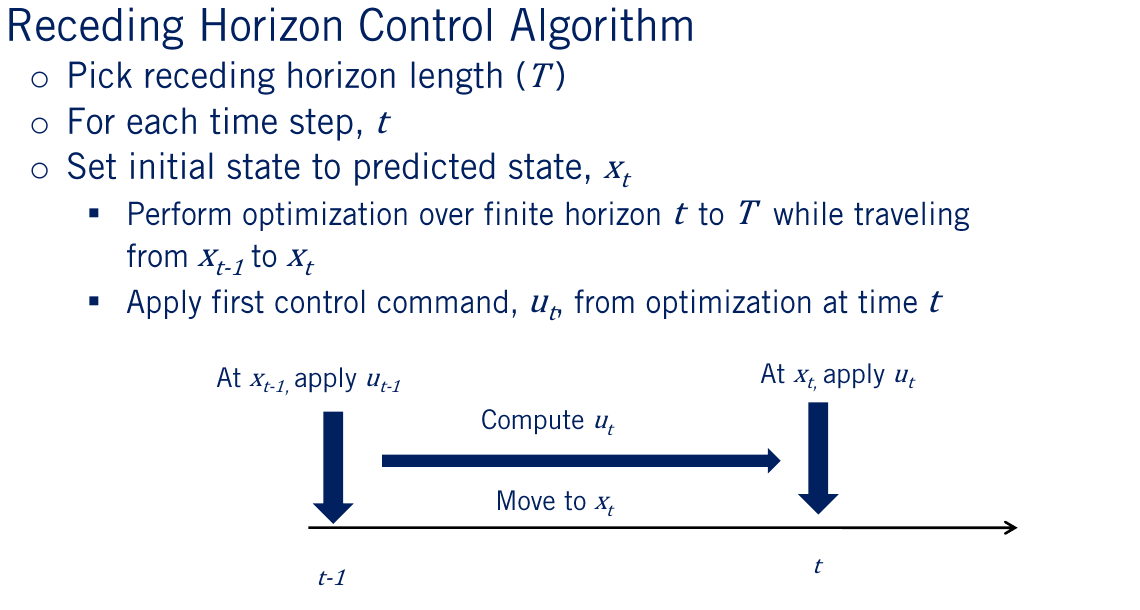
\includegraphics[scale=0.280]{img/lateral_control/mpc_1.jpeg}
\end{center}
\caption{Receding horizon algorithm.}
\label{mpc_1}
\end{figure}

Although we won't exactly arrive at the predicted state at
time $t$ due to disturbances, we do expect to be reasonably close
if the time interval is short. Finally, we apply the control
signal from the first time step of the receding horizon optimization and repeat the process
for the next time step. We can visualize the Receding
Horizon or MPC Algorithm, using the following block
diagram for a control. 

\begin{figure}[!htb]
\begin{center}
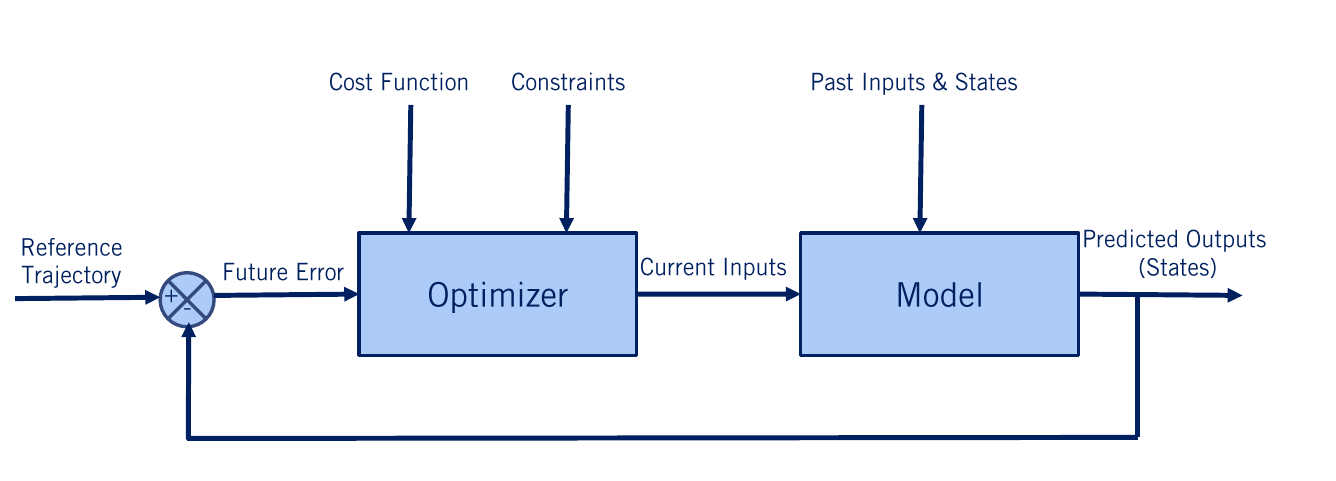
\includegraphics[scale=0.280]{img/lateral_control/mpc_2.jpeg}
\end{center}
\caption{MPC block diagram.}
\label{mpc_2}
\end{figure}

We have two main blocks,
an optimizer block, which is the core MPC component or a Receding Horizon
Control component, and the dynamic model. The model takes in
the past inputs and state from time $t-1$ and takes in the output of the optimizer which is the current sequence of inputs $U$
at each time step in the horizon. The model then outputs predicted
states at the next time-step, which are compared to
the reference trajectory and passed into the optimizer as
the future or predicted error. The optimizer also receives updated constraints and
the cost function to use, which can be fixed in advanced or varied based on changing
operating modes. The optimizer then solves its optimization and
the process repeats. 

\subsection{Linear MPC design}
\label{linear_mpc_design}

Now, let's take a look at
the linear MPC design in particular. We use the state space
formulation which represents a motion
model in discrete form. The future states
are linearly related to the current states and
the actuator signals. 

\begin{equation}
x_{t+1} = Ax_t + Bu_t
\end{equation}

Note that, $A$ and $B$ are the coefficient matrices and are
assumed to be time-invariant. MPC seeks to find a control policy $ U = \{u_{t|t}, u_{t+1|t}, u_{t+2|t}, \ldots \}$ of inputs
over a finite horizon. If all the states are
to be driven to zero, the objective function or cost
function when we minimize, can be defined as follows:

\begin{equation}
J(x(t) , U) = \sum_{j=t}^{t+T-1} x_{j|t}^TQx_{j|t} + u_{j|t}^tRu_{j|t}
\end{equation}

with quadratic error on both deviations of the state from zero and on non-zero control inputs. This is similar to
the optimization problem of optimal control theory and trades off control performance and
input aggressiveness. Note that, the matrices $Q$
and $R$ are called weight matrices and can be selected to achieve a particular
type of response. If instead we need to track a reference signals such
as a desired trajectory, we modify the formulation to include the error $\delta x$ relative
to the desired state. 

\begin{equation}
\delta x_{j|t} = x_{j|t,des} - x_{j|t}, ~~ J(x(t) , U) = \sum_{j=t}^{t+T-1} \delta x_{j|t}^TQ\delta x_{j|t} + u_{j|t}^tRu_{j|t}
\end{equation}

This is a famous
optimization formulation and has a closed form solution, the Linear Quadratic Regulator or LQR. The closed form solution
uses full state feedback, meaning that all states are
used in the control response. The LQR solution defines
a control gain matrix $K$, which can be computed from
the $A$ and $B$ matrices of the state-space model and the $Q$ and $R$ matrices
of the cost function. We can write the uncostrained, finite horizon discrete time problem formulation s

\begin{eqnarray}
\text{min}_{\substack{U}}J(x(t), U) = x_{t+T|t}^TQ_fx_{t+T|t} + \sum_{j=t}^{t+T-1}  x_{j|t}^TQ x_{j|t} + u_{j|t}^TRu_{j|t} \\
\text{such that} ~~ x_{j+1|t} = Ax_{t|t} + Bu_{t|t}, ~~ t \leq j \leq t+T-1
\end{eqnarray}

\subsection{Nonlinear MPC design}
\label{nonlinear_mpc_design}

In the more general case, the objective function is any differentiable nonlinear function of a state and inputs over
the receding horizon. The constraints imposed on
the optimization can include; nonlinear dynamic models of motion, state and input bounds that capture things like
maximum steering angles, and any other inequality
constraints g are equality constraints
h that affect our system. 

For such a general optimization problem however, no closed form solution exists. Thus, we  rely on numerical
optimization to find a solution. Even the kinematic bicycle
model falls into this category. Almost all MPC controllers for autonomous driving are solved numerically. Let's now look at
the implementation of an MPC controller for trajectory
tracking on a self-driving car. 

MPC will be used in the same feedback
structure presented earlier, but we include the conversion from the tire forces to throttle, break, and steering commands as a low
level controller inside the loop. Thus, we will have the following block structure

\begin{figure}[!htb]
\begin{center}
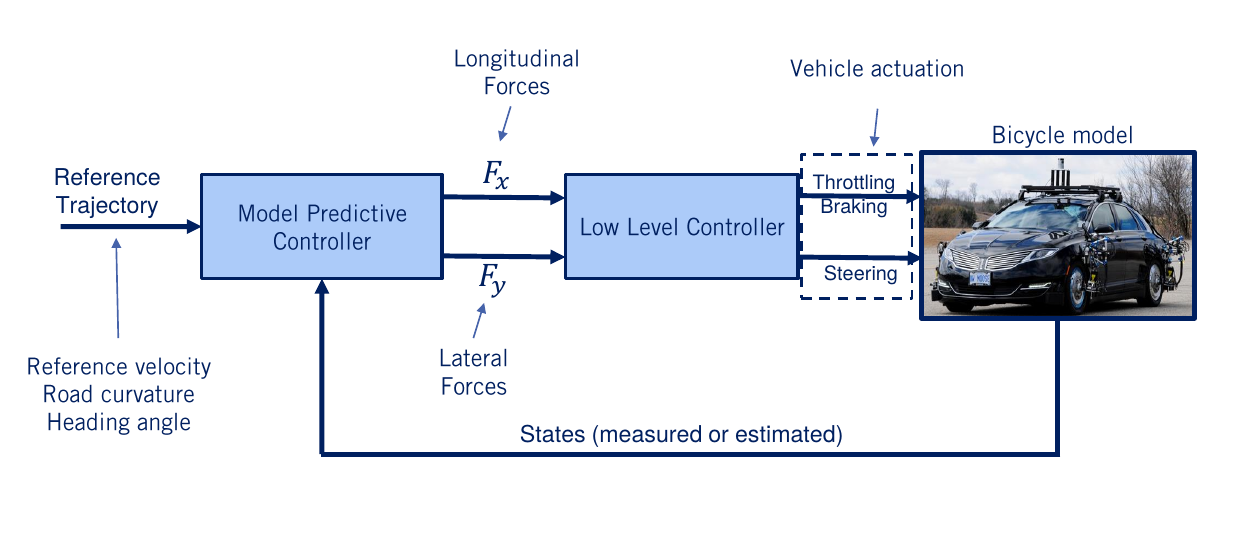
\includegraphics[scale=0.280]{img/lateral_control/mpc_3.jpeg}
\end{center}
\caption{nonlinear MPC block diagram.}
\label{mpc_3}
\end{figure}

The inputs to the MPC block
or the reference trajectory, which include the reference
path and velocity, as well as the vehicle states
at each time step. The outputs of the MPC block are the lateral and longitudinal forces needed to follow
the desired trajectory. These forces are then translated
into throttle, breaking, and steering commands, as the output
of the low-level control. Finally, the actuation signals are applied to the vehicle
at each time-step, and a new vehicle state is achieved
closing the feedback loop. 

The MPC optimization will be set up as follows to perform
a double lane change maneuver. First, we define a cost for
tracking the desired trajectory, which includes deviation from the desired trajectory and minimization of control
command magnitude. Next, we define motion
constraints on the vehicle, which rely on the lateral
and longitudinal models developed in earlier videos. We also impose maximum limits on the tire forces
to restrict them to fall within the linear tire region to avoid extreme responses
to control our errors. These costs and constraints define the optimization used in our example, which then gets converted into actual vehicle commands by
the low-level controller. It is also possible to incorporate the low-level control into
the MPC optimization, which would involve including
as constraints, the engine map, full vehicle dynamic models, actuator forces, and
tire force models. The result is a large
optimization problem that may be challenging
to solve in real time, but let's have a look at the results. 

This simulation is done for
the double lane change scenario, where the vehicle first accelerates
to a steady-state speed of $17m/s$  or $60km/h$, then maneuvers
four meters to the left, and returns four meters to
the right immediately thereafter. Plots \ref{mpc_4} and \ref{mpc_5}
show the results of the simulated maneuver
with MPC control, with the reference trajectory in blue and the actual
vehicle trajectory in red. 

\begin{figure}[!htb]
\begin{center}
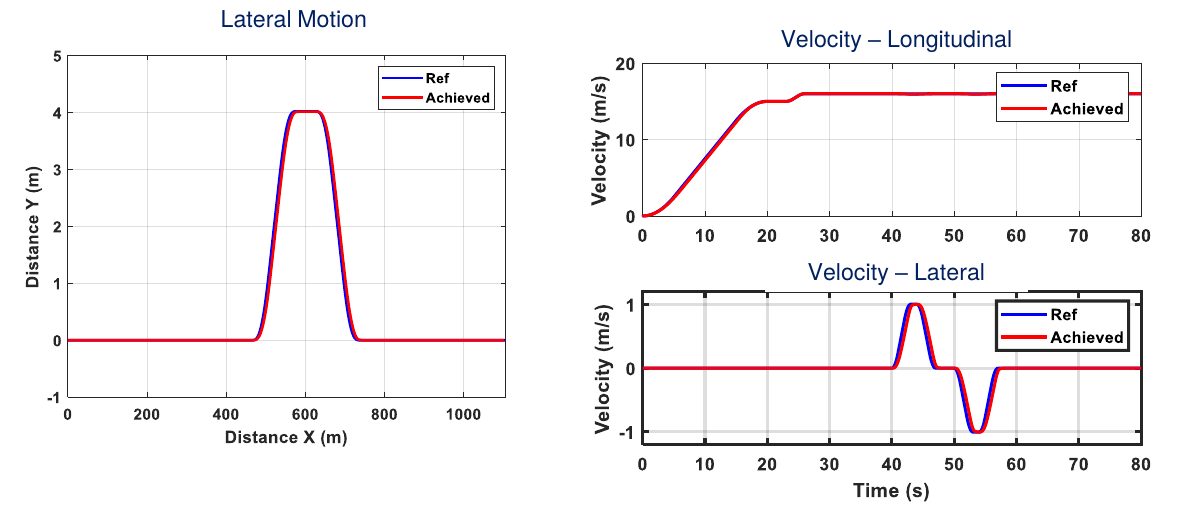
\includegraphics[scale=0.280]{img/lateral_control/mpc_4.jpeg}
\end{center}
\caption{MPC simulation.}
\label{mpc_4}
\end{figure}

\begin{figure}[!htb]
\begin{center}
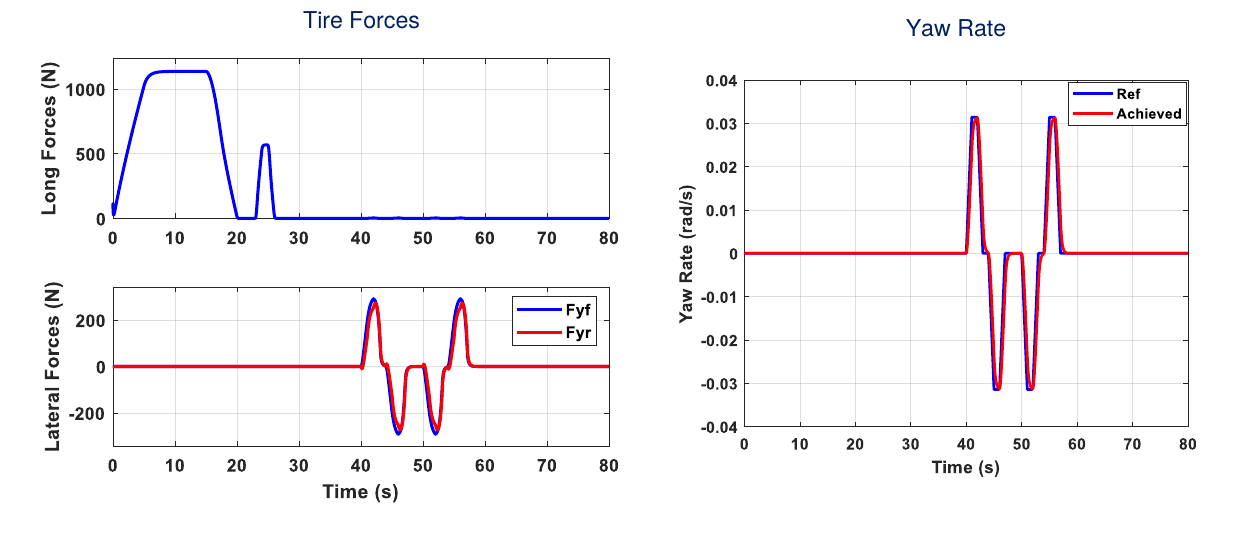
\includegraphics[scale=0.280]{img/lateral_control/mpc_5.jpeg}
\end{center}
\caption{MPC simulation.}
\label{mpc_5}
\end{figure}

We can see that
the tracking performance with the MPC controller is excellent, lagging slightly, but without
overshoot or oscillation. This is perhaps not
surprising as the simulation and MPC use the same
model and parameters. The output of model
predictive controllers, the lateral and longitudinal forces, can be seen to be smoothly
varying and well-behaved. Also, the vehicle yaw rate during the double lane change
maneuver is plotted, revealing precise tracking
throughout the states of a vehicle. MPC shows a lot of promises a control technique for
autonomous driving and can be used without modification
for a wide range of operating conditions and
a large variety of scenarios. This flexibility and
convenience comes at the cost of increased computational
requirements and relies on the availability of
robust optimization solvers to always return feasible solutions
in the available time window. 

\subsection{Questions}
\label{questions_lateral_control}

\begin{enumerate}
\item Which reference path is the most compact and easy to construct?
\begin{enumerate}
		\item Track straight line segment
		\item Track waypoints
		\item Track parameterized curves
		\item None of the above
	\end{enumerate}
	
\item What is the most ACCURATE and PRECISE definition of the crosstrack error?
	\begin{enumerate}
		\item   The crosstrack error is the difference between path heading and the vehicle heading at a reference point along the path
		\item The crosstrack error is the distance between the vehicle reference point and the closest point on the reference path
		\item The crosstrack error is the sum of the absolute difference between each coordinate of the vehicle reference point and the corresponding closest point on the desired path
		\item None of the above
	\end{enumerate}
\item What vehicle reference frame is used in a pure pursuit controller?
	\begin{enumerate}
		\item  Center of gravity
		\item Center of the front axle
		\item Center of the rear axle
		\item None of the above
	\end{enumerate}
\item Compute the radius from the instantaneous center of rotation to the center of the vehicle rear axle (in m) required for an autonomous vehicle to follow the desired path based on the information below. The lookahead distance is $10m$; the car length is $4m$; the angle between the vehicle’s body heading 
and the lookahead line is 30 degrees. Your answer should be an integer. 

\item Compute the steering angle (in degrees) required for an autonomous vehicle with pure pursuit lateral 
control for following the desired path based on the information below.
The lookahead distance is $15m$; the car length is $5m$; the angle between the vehicle’s body heading and the lookahead line is 60 degrees.

\item Consider a situation in which a vehicle traveling speed has decreased from $100km/h$ to $50km/h$. 
This vehicle lateral control is implemented with a pure pursuit controller where $l_d$​ is assigned as a function of vehicle speed. 
How should $l_d$ change in this situation?
	\begin{enumerate}
		\item  $l_d$​ should increase
		\item  $l_d$ should decrease
		\item  $l_d$​ should stay the same
		\item  $l_d$ can increase or decrease depending on how the controller is tuned
		\item None of the above
	\end{enumerate}
\item What are major components of the Stanley controller? (Select all that apply)

	\begin{enumerate}
		\item  Steering angle command is restricted to the min and max steering angles
		\item Steering angle is set equal to the heading direction to eliminate heading error relative to the path
		\item Derivative control is introduced for minimizing the heading error
		\item Proportional control is introduced for minimizing the crosstrack error
		\item Crosstrack error is eliminated
		\item Integral control is added for both the heading and the crosstrack errors optimization 
	\end{enumerate}

\item What is the correct figure of the crosstrack error dynamics for a small error value(where $\dot{e}(t)=−ke(t)$)?
\begin{figure}[!htb]
\begin{center}
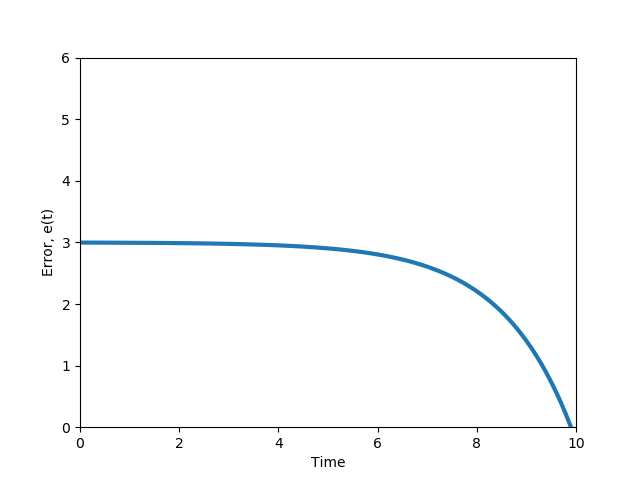
\includegraphics[scale=0.280]{img/lateral_control/error_incorrect3.png}
\end{center}
\caption{One}
\label{error_incorrect3}
\end{figure}
\begin{figure}[!htb]
\begin{center}
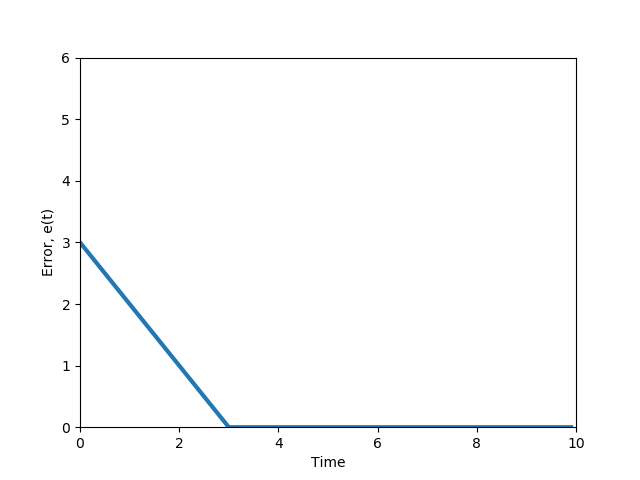
\includegraphics[scale=0.280]{img/lateral_control/error_incorrect2.png}
\end{center}
\caption{Two}
\label{Openloop}
\end{figure}
\begin{figure}[!htb]
\begin{center}
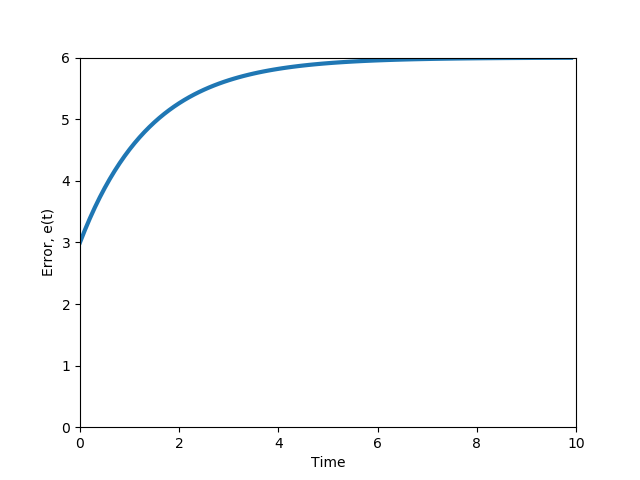
\includegraphics[scale=0.280]{img/lateral_control/error_incorrect1.png}
\end{center}
\caption{Three}
\label{Openloop}
\end{figure}
\begin{figure}[!htb]
\begin{center}
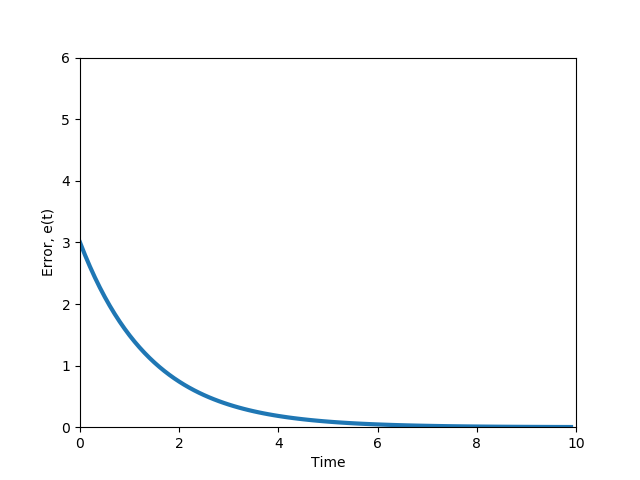
\includegraphics[scale=0.280]{img/lateral_control/error_correct.png}
\end{center}
\caption{Four}
\label{Openloop}
\end{figure}

\item What is the value of the crosstrack error, governed by the ODE 
$\dot{e}(t)=−ke(t)$, at $t=2$ given that $e(0)=4$ and $k=1$?
	
\item Which of the statements below about Model Predictive Control (MPC) are TRUE? (Select all that apply)
\begin{enumerate}
		\item    MPC works for both linear and nonlinear models
		\item MPC is an optimized version of Receding Horizon Control
		\item MPC can impose constraints on the states and the input simultaneously
		\item The formulation of an MPC controller is straightforward 
	\end{enumerate}
\item What is the typical way of finding the solution for a nonlinear vehicle dynamics model given an input functionn
\begin{enumerate}
		\item  Laplace transform
		\item Numerical optimization
		\item Using existing closed form solution
		\item None of the above 
	\end{enumerate}
\item What is the output of the Model Predictive Controller described in this course? (Select all that apply) 
\begin{enumerate}
		\item Throttling/braking
		\item Steering angle
		\item Longitudinal forces
		\item Lateral forces
		\item None of the above
	\end{enumerate}

\end{enumerate}


